\documentclass{beamer}
\setbeamertemplate{navigation symbols}{}
\usetheme{Malmoe}
\usecolortheme{beaver}

%\beamertemplatenavigationsymbolsempty
\beamersetuncovermixins{\opaqueness<1>{25}}{\opaqueness<2->{15}}

%\usepackage{float}
\usepackage{amssymb}
\usepackage{wrapfig}
\usepackage{amsmath}
\usepackage[ngerman]{babel}
\usepackage[utf8]{inputenc}
\usepackage{float}
\usepackage{graphicx}
%\usepackage{wrapfig}
\usepackage{textcomp}
\usepackage{braket}
\usepackage{bbm}
\usepackage{framed}
\usepackage{bbold}
\usepackage{colortbl}
\usepackage{color}
\usepackage{ifthen}
%\usepackage{setspace}
\newcommand{\tikzfig}[2]{\begin{figure}[h]\begin{center}\input{./img/TikZ/#1.tex}\end{center}\end{figure}}
\newcommand{\tikzfigC}[2]{\begin{figure}[h]\begin{center}\input{./img/TikZ/#1.tex}\end{center}\caption{{#2}}\end{figure}}
\newcommand{\fig}[2]{\begin{figure}[h]\begin{center}\includegraphics[width = 0.5\textwidth]{./img/#1}\end{center}\caption{{#2}}\end{figure}}
\usepackage[T1]{fontenc}
\usepackage{amsthm}
\usepackage{bm}
\usepackage{amsbsy}
\usepackage{tikz,pgfplots}
\usepackage{xcolor}
\usepackage{scalefnt}
\usepackage{caption}


\usetikzlibrary{calc,arrows,external,shapes,shapes.multipart}
%\tikzexternalize[prefix=figures/]


\addto\captionsngerman{
\renewcommand{\figurename}{Figure}%
\renewcommand{\tablename}{Tab.}%
}
\setlength{\parskip}{1.5ex plus0.5ex minus0.5ex}
\setlength{\parindent}{0em} 

\sloppy \frenchspacing \raggedbottom 

\begin{document}
%\part{ABS}
\title{Sampling the Ising Model}
\author{Abraham Hinteregger}
\institute{University of Vienna}
\date{04.10.2013}
\titlepage
\setcounter{tocdepth}{4}
%\AtBeginSection[]{
%\begin{frame}
%\frametitle{Chapter} 
%\tableofcontents[currentsection,currentsubsection,currentsubsubsection,hideothersubsections]
%\end{frame}
%}
\section{Model} 
\subsection{History}
\begin{frame}\frametitle{History} 
%\begin{block}{}
\begin{itemize}%[<+->]
\item Proposed by Wilhelm Lenz to his student Ernst Ising
\item 1924: \href{http://link.springer.com/content/pdf/10.1007 BF02980577.pdf}{Ernst Ising - \textit{Beitrag zur Theorie des Ferromagnetismus}\footnote{Zeitschrift für Physik Februar–April 1925, Volume 31, Issue 1, pp 253-258 }}
\begin{quote}
''Es entsteht \ldots [durch] \ldots die Beschr"ankung der Wechselwirkung auf diejenige  benachbarter Elemente [\ldots] kein Ferromagnetismus.''
\end{quote}
\item 1936: \href{http://journals.cambridge.org/action/displayAbstract?fromPage=online\&aid=2027260}{Rudolph Peierls - \textit{On Ising's model of ferromagnetism}\footnote{Cambridge Philosophical Society 1936, Volume 32, Issue 03, Oct.}}
\begin{quote}
''[\ldots] for sufficiently low temperatures the Ising model in two [or more] dimensions shows ferromagnetism [\ldots].
\end{quote}
\end{itemize}
%\end{block}
\end{frame}

%:TODO
%:\subsection{Phase Transitions}\begin{frame}\frametitle{Phase Transitions}
%\end{frame}%1st 2nd order - macro/microscopic differences, discontinuity


\subsection{Lattice Geometry}
\begin{frame}\frametitle{Lattice}
\tikzfigC{Ising1D}{Square Lattice in 1 dimension}
\vspace*{0.25cm}
\tikzfigC{Ising2D}{Square Lattice in 2 \alt<9-10>{and 3 }{}dimensions}
\end{frame}

\subsection{Lattice Sites}
\begin{frame}\frametitle{Lattice Sites}
\begin{itemize}
\item Each site has a state $s_i = -1\lor1$
\visible<2->{\item Assignment of states $S = (s_0, s_1, s_2,\ldots, s_{N-1})$ to the lattice sites is called a configuration
\item Therefore $2^N$ unique configurations for a lattice with N lattice sites.}
\end{itemize}
\end{frame}





\subsection{Magnetization}
\begin{frame}\frametitle{Magnetization}
\begin{itemize}
\item The magnetization of a configuration is calculated by \[M_S = M(S) = \sum_i^N s_i \in[-N,N]\]
\item The squared magnetization is an indicator for the degree of order \[M_S^2 = \sum_i s_i^2 \in[0,N]\]
%:TODO Grad der Ordnung
\end{itemize}
\end{frame}



\subsection{Energy}
\begin{frame}\frametitle{Energy}
\begin{itemize}
\item Each configuration has a corresponding energy - the Hamiltonian.
\visible<1->{
\begin{equation*}E_S = E(S) = H(s_0, s_1,\ldots, s_{N-1})=
	\alert<3>{ -J \sum_{\text{<i,j>}}s_i\cdot s_j}
	\alert<2>{- h \sum_{\text{i}}s_i}
	\end{equation*}
}
\end{itemize}\end{frame}
\begin{frame}
\begin{equation*}
H_S = -J \sum_{\text{<i,j>}}s_i\cdot s_j\qquad\in[-2NJ,2NJ]
\end{equation*}\tikzfigC{Examples}{Energy contribution (nearest neighbor interaction) of the bonds connected to the central lattice site}
\end{frame}

\begin{frame}
\frametitle{Boltzmann distribution}
 Probability of system being in the state S is given by the Boltzmann distribution ($\beta = 1/kT$) \[p_S = p(S) =\frac{ e^{-\beta E_S}}{Z}\]
 Z is the the partition function\[Z = \sum_i^{2^N} e^{-\beta E_{S_i}}\]
\end{frame}

\section*{}
\begin{frame}
\begin{itemize}
\item Calculating all $2^N$ possible configurations (or a big part of them) only viable for small systems.
\item Sampling from random configurations would lead to many high- energy (temperature) configurations (simple sampling)
\end{itemize}
\visible<2->{
$\rightarrow$ \textit{importance sampling}
}

\end{frame}

\section{Markov Chain Monte Carlo}

\subsection{Markov Chain}
\begin{frame}
\frametitle{Markov Chain}
\begin{itemize}
\item Chain of iteratively created configurations $C_1, C_2, \ldots C_n$
\item Resulting configurations correspond to the desired probability distribution $p$ and span the entire state space.
\item Configuration $C_t$ only depends on $C_{t-1}$ (Markov property).
\end{itemize}
\end{frame}

\subsection{Transition probability}
\begin{frame}
\frametitle{Transitions in the Markov Chain}
\begin{align*}
&\text{Probability for being in state A: }	&& p_A\\
&\text{Transition probability for transition $S_A \rightarrow S_B$:} &&p_{AB}\\
\end{align*}
If it fulfills \textit{detailed balance} (it must!)
\begin{align*}
 p_A\cdot p_{AB} &= p_B\cdot p_{BA}\\
\intertext{the following relation for the transition probability follows:}
\frac{p_{AB}}{p_{BA}} = \frac{p_B}{p_A} &= \left(\frac{Z}{Z}\right)\frac{e^{-\beta E_B}}{e^{-\beta E_A}}  = e^{-\beta (E_B - E_A) = e^{-\beta \Delta E}}
\end{align*}
\end{frame}


\subsection{Metropolis Hastings Algorithm}
\begin{frame}\frametitle{Metropolis- Hastings Algorithm}
\begin{itemize}
\item Configuration after t steps is $C_t$
\item Flip one lattice site $\rightarrow$ $C_t'$
\begin{itemize}
\item  has to be chosen randomly - suitable RNG necessary
\end{itemize}
\item Calculate energy difference $\Delta E = E_t' - E_t$
\item Calculate acceptance probability $P$
\begin{equation*}
P = \operatorname{min}\left(1,e^{-\beta\cdot \Delta E}\right),\qquad \beta = 1/kT > 0 
\end{equation*}
\item Generate random number $r \in [0,1[$
\begin{itemize}
\item $r<P \rightarrow C_{t+1} = C_t'$ 
\item $r>P \rightarrow C_{t+1} = C_t$ 
\end{itemize}
\end{itemize}
\end{frame}

\subsection{Results}% 75x75 Swendsen Wang
\begin{frame}
\frametitle{Absolute magnetization per spin}
\begin{minipage}{0.70\textwidth}
\begin{tikzpicture}[scale=0.85]
\begin{axis}[xmax=3,ymax=1,ymin=0,grid=major,
xlabel={T},
ylabel={|M|},
extra x ticks={2.267},
extra x tick labels={$T_c$}]
\begin{scope}
\addplot[mark=+,mark options={black}, white]coordinates{(1.75,1)};\label{plot:mcB}
\addplot[mark=+,mark options={white}, white]coordinates{(1.75,1)};
\end{scope}
\only<1-2>{\addplot[mark=o,mark options=blue,white] coordinates {
(1.00,1)
(1.20,1)
(1.40,0.99)
(1.60,0.98)
(1.70,0.97)
(1.80,0.957)
(1.90,0.937)
(2.00,0.91)
(2.05,0.89)
(2.10,0.87)
(2.15,0.84)
(2.20,0.783)
(2.225,0.74)
(2.25,0.67)
(2.2692,0.54)
(2.275,0.48)
(2.30,0.39)
(2.35,0.20)
(2.40,0.13)
(2.45,0.10)
(2.50,0.08)
(2.60,0.045)
(2.70,0.03)
(2.80,0.027)
(2.90,0.026)
(3.00,0.025)};\label{plot:mc}}
\only<2>{\addplot[mark=+,mark options={black}, white] coordinates {
(1.00,1)
(1.20,1)
(1.40,0.99)
(1.60,0.98)
(1.70,0.97)
(1.80,0.957)
(1.90,0.938)
(2.00,0.907)
(2.05,0.893)
(2.10,0.871)
(2.15,0.84)
(2.20,0.784)
(2.225,0.745)
(2.25,0.687)
(2.2692,0.62)
(2.275,0.585)
(2.30,0.493)
(2.35,0.303)
(2.40,0.213)
(2.45,0.152)
(2.50,0.126)
(2.60,0.100)
(2.70,0.07)
(2.80,0.068)
(2.90,0.06)
(3.00,0.05)};}
\only<2-1>{\addplot[mark=triangle,mark options={black}, white] coordinates {
(2.3,0.730)
(2.3,0.638)
(2.3,0.589)
(2.3,0.537)
(2.3,0.483)
(2.3,0.449)
(2.3,0.413)
(2.3,0.390)
(2.3,0.357)
(2.3,0.318)
(2.3,0.362)
(2.3,0.242)
};}
\addplot[line width=1pt,red,samples = 500,domain=1.001:5]
	{(1-sinh(2/(x))^(-4))^(0.125)};\label{plot:analytical}
\addplot[red,line width= 1pt] coordinates {(2.267,0.55)(2.267,0)(3,0)};


\end{axis}
\end{tikzpicture}
\end{minipage}\begin{minipage}{0.25\textwidth}
\visible<2->{\ref{plot:mcB} MC $50\times 50$}

\ref{plot:mc} MC $75\times 75$

\ref{plot:analytical} analytical
\end{minipage}
\end{frame}

\begin{frame}
\frametitle{Magnetization over time}
\begin{figure}[h]\begin{center}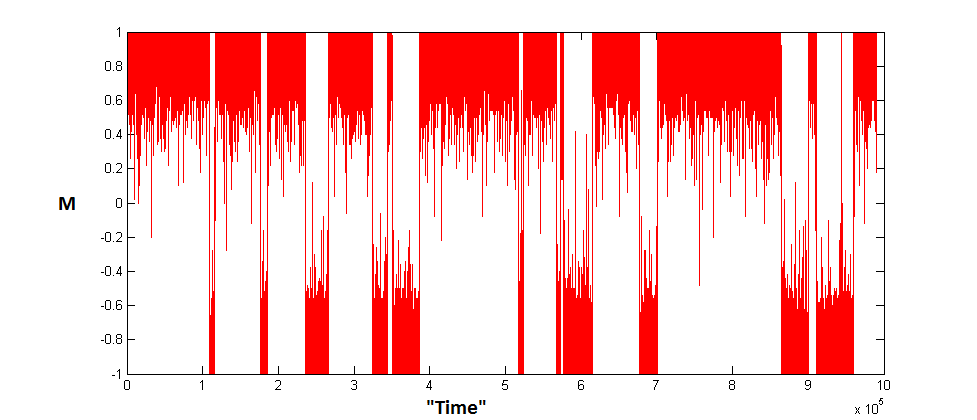
\includegraphics[width = \textwidth]{./img/MPlot.png}\end{center}\caption{M per spin plotted over time (Monte Carlo steps)}\end{figure}
\end{frame}

%: TODO Autocorrelation transition folie

\section{Autocorrelation}
\subsection{}






\begin{frame}\frametitle{Properties of a configuration s}
\begin{itemize}
\item Energy -- Hamiltonian: $E(s) = H(s)$
\item  Internal energy (per spin): $e(s) = E/N \in [ -2,2]$
\item Magnetization: $M(s) = \sum_i^N s_i$
\item Magnetization (per spin): $m(s) = M/N\in [ -1,1]$
\end{itemize}
\end{frame}



\section{Dynamics}
\subsection{Temperature}
\begin{frame}\frametitle{Temperature}
%:TODO
\end{frame}


\begin{frame}\frametitle{Temperature in the Ising Model}
\begin{equation*}
P = \operatorname{min}\left(1,e^{-\beta\cdot \Delta H}\right),\qquad \beta = 1/kT > 0
\end{equation*}
\begin{itemize}
\item $\Delta H < 0 \rightarrow P = 1$
\item high temperature leads to higher acceptance probability
$\rightarrow$ unordered (low magnetization, Curie Temperature $T_c$)
\item critical temperature $T_c$ when $\left<\sum_i^N s_i\right>/N \approx 0$
\visible<2->{\begin{itemize}
\item $kT_c/J = 2.269$
\end{itemize}}
\end{itemize}
\end{frame}




\subsection{Cluster Flip Algorithms}
\begin{frame}\frametitle{Cluster Flip Algorithms}

\end{frame}
\subsection{Time}






%: ??????????????
%%%%%%%%%% ?
\section{Stuff}
\subsection{Summary}
\begin{frame}\frametitle{Summary - Ising Model}
\begin{itemize}
\item molecules on a lattice - each with with one of two possible states
\item (magnetic) moments prefer to align
\item low temperatures: ordered
\item high temperatures: disordered
\end{itemize}
\end{frame}
\subsection{Different Models}\begin{frame}\frametitle{Different Models}\end{frame}%Potts blablbal - only 2 state Ising here blabla


\begin{frame}
\begin{itemize}
\item Single value obtained from one configuration hasn't much significance
\item Average from many (n) configurations instead:
\begin{align*}
\bar{E } = \frac{1}{n}\sum_i^n E_{S_i} && \bar{M } = \frac{1}{n}\sum_i^n M_{S_i}&&\ldots 
\end{align*}
\alert<2>{\visible<2->{\item Sampling from completely random configurations does not work well for ordered configurations seen in ferromagnets.}}
\end{itemize}
%: Notwendigkeit von gewisser Wahrscheinlichkeitsverteilung vllt andeuten
\end{frame}







\end{document}%%%%%%%%%%%%%%%%%%%%%%%
%%%%%%%%%%%%%%%%%%%%%%%%%%%%%%
%%%%%%%%%%%%%%%%%%%%%%%%%%%%%%
%%%%%%%%%%%%%%%%%%%%%%%%%%%%%%
%%%%%%%%%%%%%%%%%%%%%%%%%%%%%%
%%%%%%%%%%%%%%%%%%%%%%%%%%%%%%
%%%%%%%%%%%%%%%%%%%%%%%%%%%%%%
%%%%%%%%%%%%%%%%%%%%%%%%%%%%%%
%%%%%%%%%%%%%%%%%%%%%%%%%%%%%%
%%%%%%%%%%%%%%%%%%%%%%%%%%%%%%
%%%%%%%%%%%%%%%%%%%%%%%%%%%%%%
%%%%%%%%%%%%%%%%%%%%%%%%%%%%%%
%%%%%%%%%%%%%%%%%%%%%%%%%%%%%%
%%%%%%%%%%%%%%%%%%%%%%%%%%%%%%
%%%%%%%%%%%%%%%%%%%%%%%%%%%%%%
%%%%%%%%%%%%%%%%%%%%%%%%%%%%%%

%: IGNORE
\section{Nucleation}
\subsection{What is Nucleation?}
\begin{frame}\frametitle{Nucleation}
\begin{itemize}
\item is a phase transformation process
\item phase transformation grows from small nucleus
\begin{exampleblock}{Examples}
\begin{itemize}
\item cloud chamber
\item \href{http://www.youtube.com/watch?v=pTdiTe3x0Bo}{supercooled water}
\end{itemize}
\end{exampleblock}
\end{itemize}
\end{frame}


\subsection{Homogeneous  Nucleation}\begin{frame}\frametitle{Nucleation}
\begin{itemize}
\item
Homogeneous nucleation
\begin{itemize}
\item in a uniform substance
\item no nucleation until nucleus with critical size ''appears'' (due to stochastic processes)
\item higher supersaturation leads to smaller critical radius.
\item rarely occurs in nature
\end{itemize}
\item Heterogeneous Nucleation{}
\begin{itemize}
\item begins at some preferable interface and grows from there
\item much (!) more likely
\item common in nature (freezing (in most cases), bubbles in water,...)
\end{itemize}
\end{itemize}
\end{frame}


\subsection{Heterogeneous  Nucleation}
\begin{frame}\frametitle{Nucleation}
\begin{itemize}
\item
Homogeneous nucleation
\begin{itemize}
\item in a uniform substance
\item no nucleation until nucleus with critical size ''appears'' (due to stochastic processes)
\item higher supersaturation leads to smaller critical radius.
\item rarely occurs in nature
\end{itemize}
\item Heterogeneous Nucleation{}
\begin{itemize}
\item begins at some preferable interface and grows from there
\item much (!) more likely
\item common in nature (freezing (in most cases), bubbles in water,...)
\end{itemize}
\end{itemize}
\end{frame}

\section{Nucleation in the Ising Model}
\subsection{Homogeneous Nucleation}
\begin{frame}{Homogeneous Nucleation in the Ising Model}
%: ÜBERARBEITEN
\begin{itemize}
\item Necessary modifications:\begin{itemize}
\item none\\
\end{itemize}\end{itemize}\begin{itemize}
\item Problems
\begin{itemize}
\item long time until nucleus of critical size appears 
\item inefficient to simulate billions of cycles until phase change takes place
\end{itemize}
\end{itemize}
\end{frame}


\begin{frame}\frametitle{Cluster size}
\fig{nsize.png}{Propability of finding a cluster of size N at different times\footnote{\href{http://www.ncbi.nlm.nih.gov/pubmed/16494425}{Pan, Rappl, Chandler, Balsara: J. Phys. Chem. B 2006}}}
\end{frame}


%: NACH HOMOGENER NUKLEATION TPS EINFÜGEN
\subsection{Transition Path Sampling}
\begin{frame}\frametitle{Transition Path Sampling (TPS) - ''shooting'' method\footnote{aa\href{http://dx.doi.org/10.1063\%2F1.476378}{Dellago, Bolhuis, Chandler: Advances in Chemical Physics 123 (1998)}}}
\begin{itemize}
\item needs two stable states (A \& B)
\item path through configuration space connecting these
\item change the path a little at a random point between A and B
\item sample new path and accept if it connects A with B
\end{itemize}
\end{frame}

\begin{frame}
\frametitle{Transition Path Sampling}
\fig{tps}{First path (red), slightly changed and accepted path (blue), rejected path (green)\footnote{\href{dx.doi.org/10.1088/0953-8984/21/33/333101}{Esobedo, Borrero, Araque - J. Phys.: Condens. Matter 21 (2009)}}}
\end{frame}


\subsection{Heterogeneous Nucleation}
\begin{frame}\frametitle{Heterogeneous Nucleation}
\begin{itemize}
\item Necessary modifications:\begin{itemize}
\item handle boundaries in heterogeneous nucleation
\begin{equation*}
H(s)= \color{gray}{ -J \sum_{\text{<i,j>}}s_i\cdot s_j - h \sum_{\text{i}}s_i}\color{black} - J_s \sum_{\text{<i,j>}}^{\text{II}}s_i\cdot s_j
\end{equation*}
\item implement walls/surfaces with fixed spins
\end{itemize}
\end{itemize}
\end{frame}


\begin{frame}\frametitle{Nucleation in and out of Pores\footnote{Page, Sear - Heterogeneous Nucleation in and out of Pores PRL 97, 065701 (2006)}}
\alt<2>{\fig{upspins}{2 phases of nucleation}}{
\begin{equation*}
H(s)= { -0.8 \sum_{\text{<i,j>}}s_i\cdot s_j - 0.05 \sum_{\text{i}}s_i}\color{gray} - 0 \sum_{\text{<i,j>}}^{\text{II}}s_i\cdot s_j,\color{black}\qquad kT = 1
\end{equation*}
\begin{itemize}
\item nucleation near surfaces $10^{12}$ times faster
\item fastest in pores
\item nucleation in 2 steps
\item diversified pore sizes lead to fastest reaction as probability of existence optimal pore size is higher
\end{itemize}}
\end{frame}


\begin{frame}\frametitle{Problems}
\begin{itemize}
\item phase transitions are rare events (with realistic values for the coupling constant, ...)
\item nonequilibrium systems therefore TPS (transition path sampling) not applicable.
\alert<2->{\visible<2->{\item $\rightarrow$ Forward Flux Sampling}}
\end{itemize}
\end{frame}


\subsection{Forward Flux Sampling}
\begin{frame}
\frametitle{Forward Flux Sampling}
\begin{itemize}
\item Similar to TIS (transition interface sampling - a modified TPS)\begin{itemize}
\item initial state A: $\lambda < \lambda_A = \lambda_0$
\item final state B:\quad\!\!\! $\lambda > \lambda_B = \lambda_n$
\item path has to pass every $\lambda_i$ in increasing order (can go backwards in between too) until it reaches $\lambda_n$ (B)
\end{itemize}
\item after reaching a new interface ($\lambda_{i+1}$) configuration is stored
\item stored configurations used as starting point for new trial runs
\item trial runs continued until path reaches A ($\rightarrow$ failure) or a new interface $\lambda_{i+1}$ ($\rightarrow$ success)
\end{itemize}
\end{frame}

\begin{frame}
\frametitle{(Direct) Forward Flux Sampling\footnote{\href{iopscience.iop.org/0953-8984/21/46/463102}{Allen, Valeriani, Rein ten Wolde: 2009 J. Phys.: Condens. Matter 21}}}
\only<1>{\fig{DFFS1}{Sampling path starting in A - store configurations where the path leaves A (X)}}
\only<2>{\fig{DFFS2}{Sampling new paths from every stored configuration. Discard if path goes back to A}}
\end{frame}


%!RATE CONSTANTS

\section{Outlook}\subsection{Possible Adjustments}
\begin{frame}
\frametitle{Possible Adjustments to the Ising Model}
\begin{itemize}
\item next-nearest neighbor interaction or even higher range
\item forces from the outside, e.g. gravity
\item Multi Hit Swendsen Wang algorithm
\item Kawasaki Dynamics (alternative Metropolis algorithm with fixed state ratios and amounts)\begin{itemize}
\item choose any (A-B) bond
\item $(A-B) \rightarrow (B-A)$
\item calculate new energy
\item \ldots
\end{itemize}
\end{itemize}
\end{frame}
\subsection{Potts Model}
\begin{frame}
\frametitle{Potts Model}
\begin{itemize}
\item states not only $-1 \land 1$ but (discrete) angles.
\item $H = -J_c \sum_{i,j}cos\left(\theta_i -\theta_j\right) +  \ldots$
\item Applications
\begin{itemize}
\item percolation (Wu: ''Percolation and the Potts Model'' (1978))
\item flow of foam (Sanyal, Soma: ''Viscous instabilities in flowing foams'' (2006))
\item cancerous tumors (Sun, Chang, Cai: ''A Discrete Simulation of Tumor Growth Concerning Nutrient Concentration'' (2004))
\end{itemize}
\end{itemize}
\end{frame}

\section{}
\subsection{Additional Literature}
\begin{frame}
\begin{itemize}
\item Page, Sear - Heterogenous Nucleation in and out of Pores (2006): PRL 97, 065701
\item Allen, Valeriani, Rein ten Wolde - Forward Flux Sampling for rare event simulations (2009): J. Phys.: Condens. Matter 21 (2009) 463102 (21pp)
\item Allen, Frenkel, Rein ten Wolde - Forward Flux Sampling-type schemes for simulating rare events: Efficiency analysis (2008): http://arxiv.org/abs/cond-mat/0602269v1
\item Escobedo, Borrero, Araque -  Transition path sampling and forward flux sampling. Applications to biological systems 2009 J. Phys.: Condens. Matter 21 333101
\end{itemize}
\end{frame}
\subsection{Simulation}
\begin{frame}
\begin{itemize}
\item Sourcefiles and binaries on my github \href{https://github.com/oerpli/Ising2D}{https://github.com/oerpli/Ising2D}
\end{itemize}
\end{frame}


\end{document}